\chapter{MIP Timing Detector (MTD)}
\section{Introduction}

In the coming years the LHC will be working toward upgrades that will lead a substantial increase in luminosity.  The timeline for future operations of the LHC is shown in Figure \ref{fig:lhctimeline}.  In 2019 the LHC entered a two-year shutdown, Long Shutdown 2 (LS2).  Upgrades of the LHC injector complex to increase the beam brightness will take place during this shutdown.  After LS2 the LHC will enter Run 3 which will run for three years at 13-14 TeV.  At the completion of Run 3 the LHC will enter Long Shutdown 3 (LS3) which will last approximately 2.5 years.  During LS3 the optics in the interaction region will be upgraded to produce smaller beams at the interaction point.  The completion of this upgrade will usher in the High Luminosity (HL-LHC) era or Phase 2 of LHC operations, during which the combination of brighter beams and a new focusing scheme at the IP allows for a potential luminosity of 2x10$^{35}$ cm$^{-2}$s$^{-1}$ at the beginning of each fill \cite{Apollinari:2017cqg}.  

\begin{figure}[h]
	\centering
	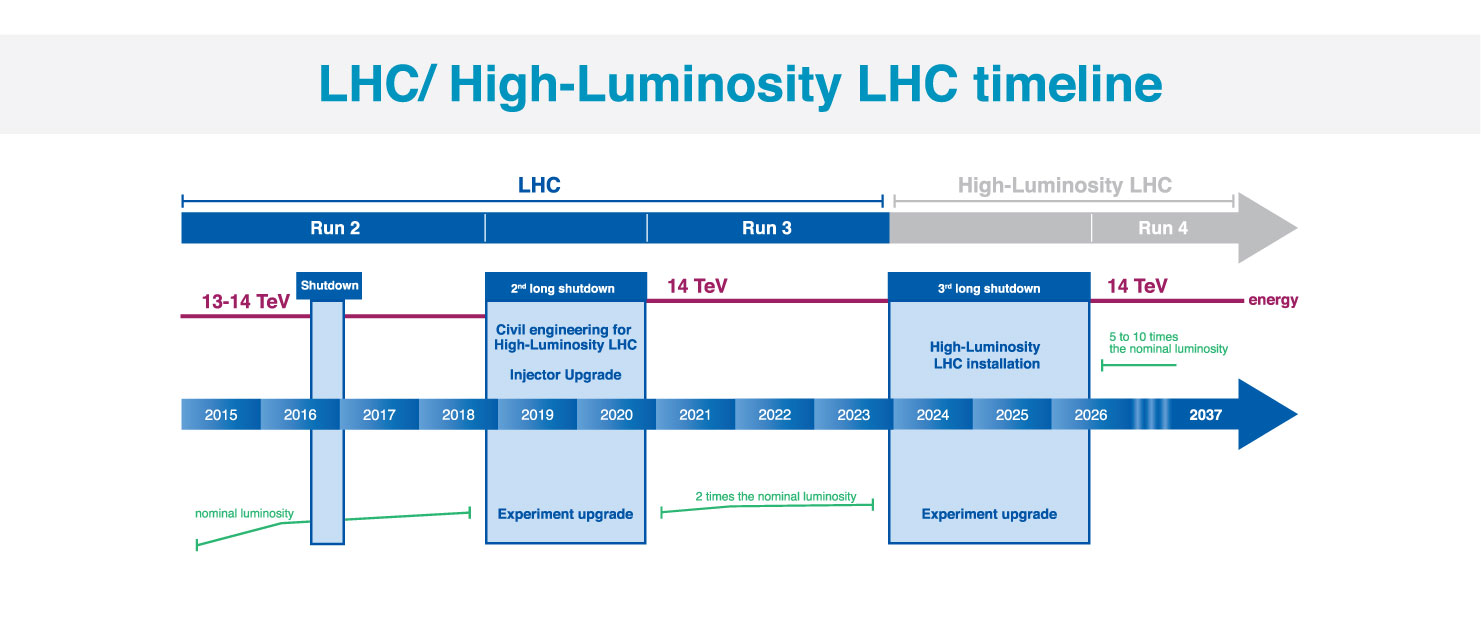
\includegraphics[width=1.0\linewidth]{Figures/LHCTimeline}
	\caption[Timeline for LHC]{Timeline for LHC \cite{DeMelis:2063307}}
	\label{fig:lhctimeline}
\end{figure}

The increased luminosity results in more interactions per bunch crossing or pileup.  In order to limit the amount of pileup the experiments must disentangle to more manageable levels, the nominal scenario would be operating at a stable luminosity of $5.0\times10^{34}$ cm$^{-2}$ s$^{-1}$.  This would limit the pileup to an average of 140.  The ultimate scenario for operations would be running at $7.5\times10^{34}$ cm$^{-2}$ s$^{-1}$ which brings the average pileup up to 200.  The CMS detector in its current state is not capable of dealing with $\approx$140-200 pileup.  At this level of pileup the spacial overlaps of tracks and energy depositions would lead to a degradation in the ability to identify and reconstruct hard interactions. In order to preserve the data quality of the current CMS detector this increased pileup must be reduced to an equivalent level approximately equal to current LHC operations which is $\sim$40.  The collision vertices within a bunch crossing have an RMS spread of 180-200 ps in time.  If the beam spot were to be sliced into consecutive snap shots of 30-40 ps then the pileup levels per snapshot would be approximately 40.  The space-time reconstruction of a 200 pileup event is shown in Figure \ref{fig:mtdpileup}.  The addition of timing information to the $z$ position spreads apart the vertices that would otherwise have been merged together and indiscernible.  In order to achieve this a detector dedicated to the precise timing of minimum ionizing particles (MIPs), the MTD, will be added to the CMS detector.  



\begin{figure}[h]
	\centering
	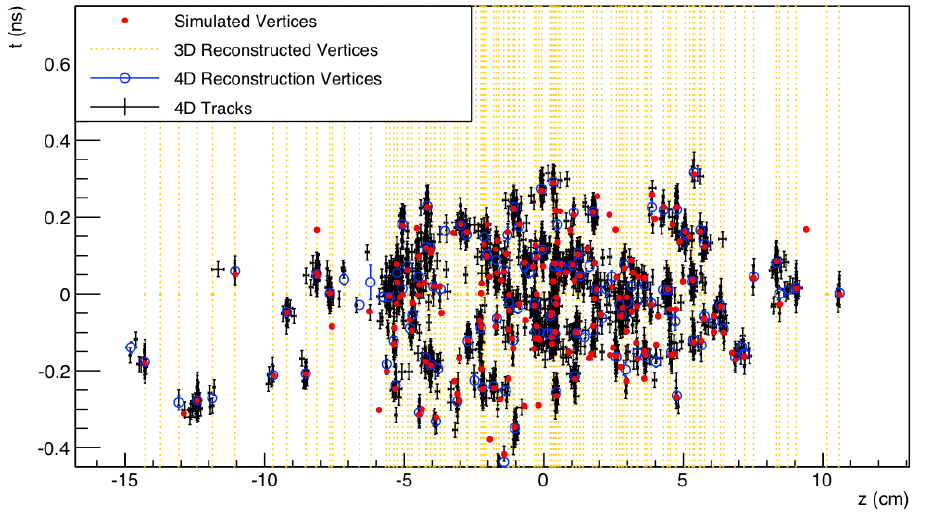
\includegraphics[width=1.0\linewidth]{Figures/MDT_pileup}
	\caption{Vertices from a simulated 200 pileup event with MTD timing resolution of $\sim$30 ps. The red dots represent the simulated vertices while the yellow lines indicate vertices reconstructed without the use of timing information. The black crosses and blue open circles represent tracks and vertices reconstructed using time information from the MTD. Reprint from}
	\label{fig:mdtpileup}
\end{figure}

\begin{figure}[h]
	\centering
	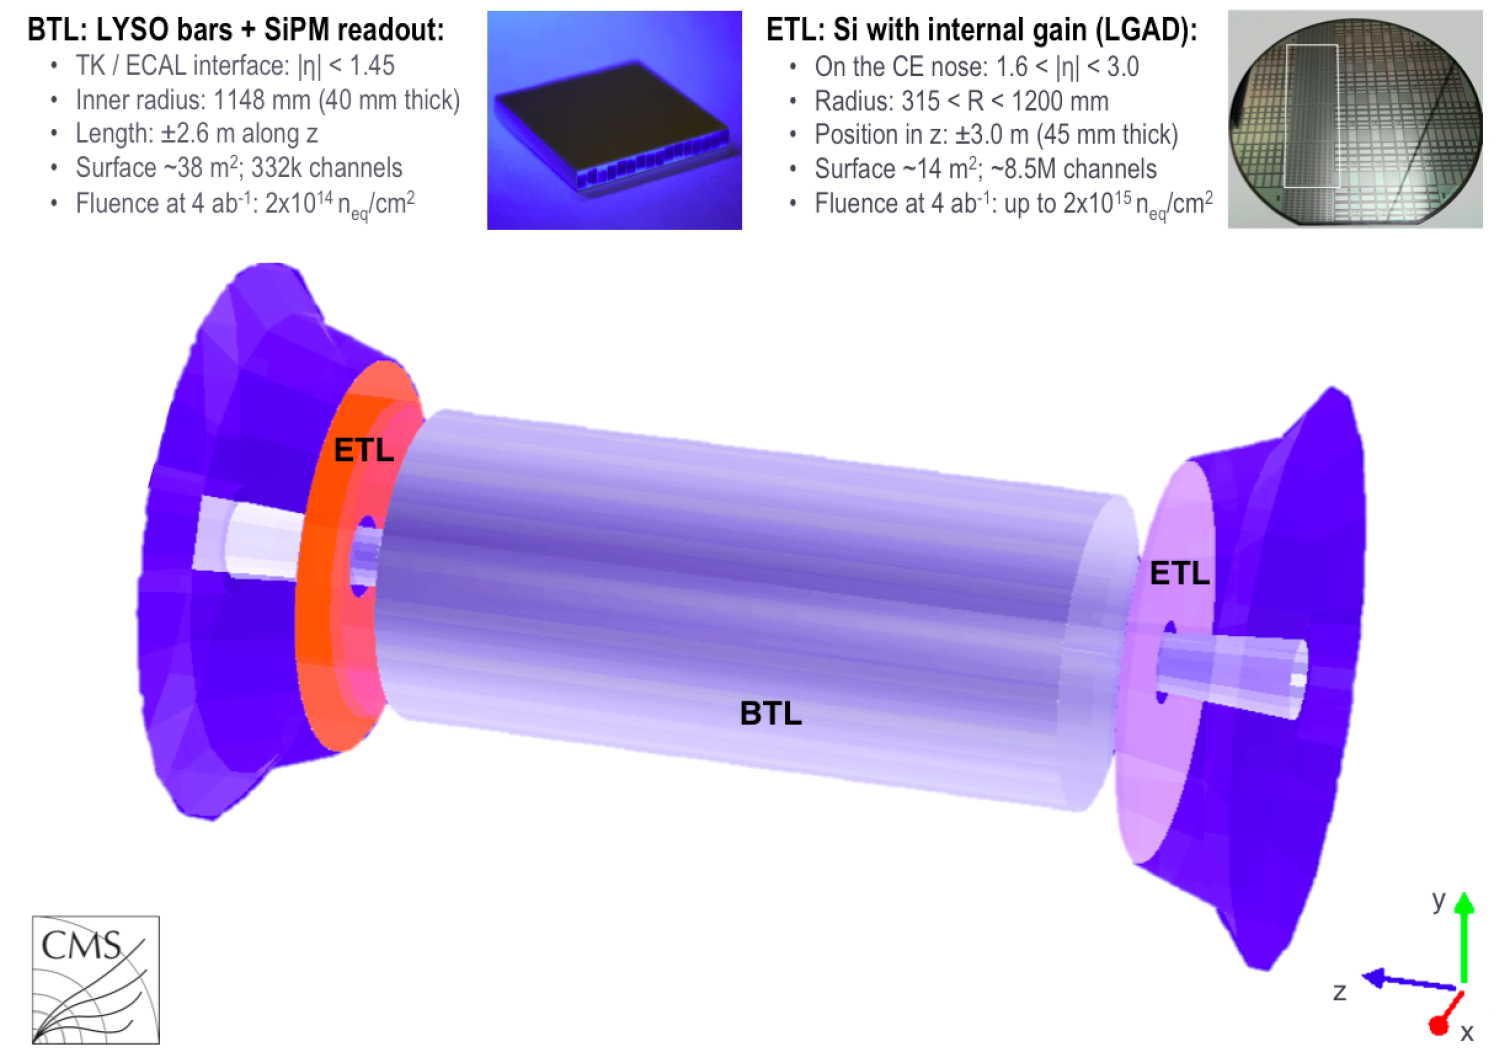
\includegraphics[width=1.0\linewidth]{Figures/MTD_overview}
	\caption[Schematic view of MTD]{Schematic view of the proposed MTD implemented in the GEANT simulation of the CMS detector. The central region makes up the BTL which will be located in the space between the tracker and the ECAL. The ETL will be located in front of the endcap calorimeter. Reprint from }
	\label{fig:mtdoverview}
\end{figure}


%The MTD will provide timing information with a resolution of 30-40 ps at the start of the HL-LHC era.  Radiation damage is expected to degrade this to 50-60 ps by the end of the HL-LHC era.


\section{Barrel Timing Layer}
 The Barrel Timing Layer (BTL) makes up the barrel region of the MTD.  It will provide pseudorapidity coverage up to $|\eta| = 1.48$ with a geometric acceptance of $\sim 90\%$.  The BTL will be capable of detecting MIPs with a time resolution of 30 ps at the start of Phase-2 operations and a luminosity-weighted time resolution of $\sim45$ ps when radiation damage effects are taken into account.  The BTL is designed to operate without significant performance degradation over an integrated luminosity of at least 3000 fb$^{-1}$.  The predicted level of radiation exposure over that integrated luminosity is listed in Table \ref{table:fluences}.
 
 \begin{table}[h]
 	\centering
 	\caption{Predicted radiation doses and fluences at different location of the BTL after an integrated luminosity of 3000 fb$^{-1}$.  The two far right columns include a safety margin of 1.5.}
 	\begin{tabular}{|c|c|c|c|c|c|c|}
 		\hline
 		& & & \multicolumn{2}{|c|}{3000 fb$^{-1}$}  & \multicolumn{2}{|c|}{$1.5\times 3000$ fb$^{-1}$}  \\
 		$|\eta|$ & $r$ (cm) & $z$ (cm) & $n_{eq}/cm^2$ & Dose (kGy) & $n_{eq}/cm^2$ & Dose (kGy) \\
 		\hline
 		\hline
 		0.0 & 116 & 0 & $1.65\times10^{14}$ & 18 & $2.48\times10^{14}$ & 27 \\
 		\hline
 		1.15 & 116 & 170 & $1.80\times10^{14}$ & 25 & $2.70\times10^{14}$ & 38 \\
 		\hline
 		1.45 & 116 & 240 & $1.90\times10^{14}$ & 32 & $2.85\times10^{14}$ & 48 \\
 		\hline
 	\end{tabular}
 \label{table:fluences}
\end{table}
 The fundamental element for MIP detection in the BTL is a thin scintillating bar made of Lutetium Yttrium Orthosilicate crystals doped with Cerium ($(Lu_{1-X}Y_X)_2SiO_5:Ce$) which is referred to as LYSO:Ce.  The bars are 57 mm long, 3.12 mm wide, and have an average thickness of 3 mm.  A silicon photomultiplier (SiPM) is attached to each end of the LYSO:Ce bar.  This double-ended readout gives uniform time response along the length of the crystal by eliminating the time delay effect from light propagating along the crystal and the ability to extract positional information for tracking. 
 
 An overview of the BTL and its components is shown in Figure \ref{fig:btloverview}.  The longitudinal axis of each crystal bar is oriented along the $\phi$-direction in the CMS detector.  The crystals are grouped in 1 $\times$ 16 ($\phi \times z$) arrays that each form a \textit{module}.  Each \textit{module} has 32 SiPMs (2 for each bar) resulting in 32 readout channels.  These \textit{modules} are then grouped in a 3 $\times$ 8 ($\phi \times z$) arrangement to make up a readout unit (RU) as shown in Figure \ref{fig:btlreadoutunit}.  Each \textit{module} is read out by a dedicated ASIC called the TOFHIR (Time-of-flight, High Rate) chip which is capable of reading out 32 channels at a time.  The TOFHIR chip gives precision timing information using discrimination of the leading edge of pulses from the SiPMs followed by a time-to-digital converter (TDC).  When using discrimination techniques like this the time for a pulse to cross the discriminating threshold depends on the height of the pulse.  This results in an amplitude-dependent timing variation called time walk.  In order to correct for this time walk effect the ASIC also measures pulse amplitude. Six ASICs are mounted on each of four front-end boards (FEBs) on a RU giving a total of 24 ASICs and 768 SiPMs per RU.  The RUs are then arranged in trays along the $z$-direction.  Each tray holds six RUs, runs along half the length of the detector, and spans $10^\circ$ along $\phi$.  To summarize, a total of 72 trays (36 azmuthal sections each split into a $+z$ and $-z$ section) contain 331776 SiPMs and 165888 LYSO:Ce bars.  This gives a detector granularity that has an average occupancy of about 7\% at 200 pileup, which limits the likelihood of multiple hits within a single crystal during a bunch crossing.  
 
 In order to have a negligible impact on the energy resolution of the ECAL, the thickness of the LYSO:Ce crystals is varied along the $z$-axis of the detector.  This variation is done in three sections such that the thickness of material is as uniform as possible while not exceeding 0.4 $X_0$ where $X_0$ is one radiation length.  This is done in three sections as a function of $\eta$ where crystal thicknesses of 3.75 mm, 3.0 mm, and 2.4 mm will be in the $|\eta|$ regions 0-0.7, 0.7-1.1, and 1.1-1.48 respectively.  These details are outlined in Table \ref{table:slantthickness}.  Figure \ref{fig:crystalslantthickness} shows how the slant thickness changes along $\eta$ in terms of radiation length for the case where crystal thicknesses are varied as outlined in Table \ref{table:slantthickness}.  
 
 \begin{table}[h]
 	\centering
 	\begin{tabular}{|l|c|c|c|}
 		\hline 
 		$|\eta|$ range & 0-0.7 & 0.7-1.1 & 1.1-1.48  \\ 
 		\hline 
 		Crystal thickness (mm) & 3.75 & 3.0 & 2.4 \\
 		\hline
 		Average slant thickness (mm) & 4.0 & 4.3 & 4.6 \\
 		\hline
 	\end{tabular} 
 	\caption{Summary of crystal and slant thicknesses in different $\eta$ regions.}
 	\label{table:slantthickness}
 \end{table}
 
 \begin{figure}[h]
 	\centering
 	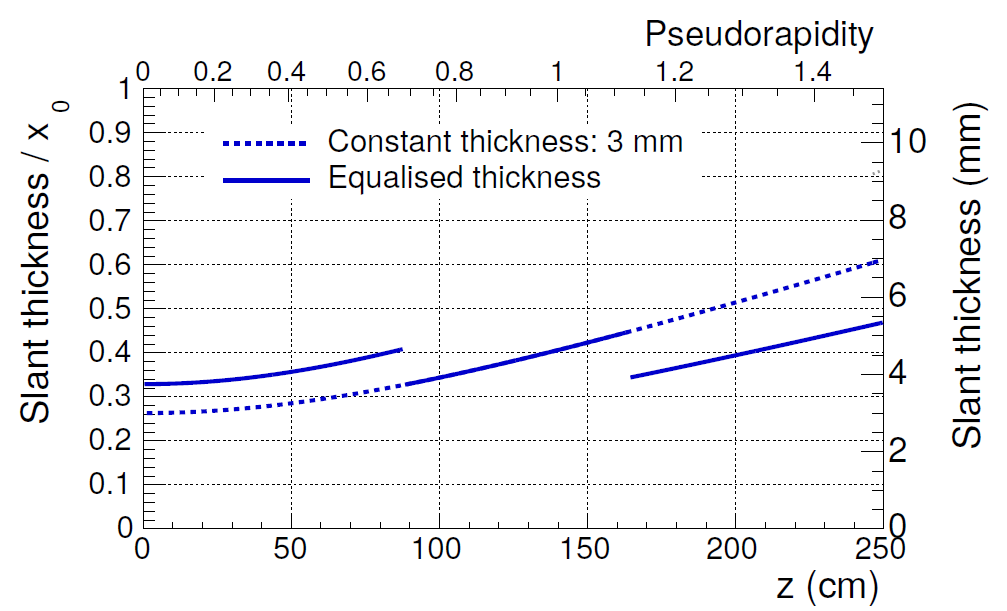
\includegraphics[width=1.0\linewidth]{Figures/crystalslantthickness}
 	\caption[LYSO:Ce crystal slant thickness in the BTL.]{The left and right axes show the slant thickness in terms of radiation length and mm respectively. The dotted blue line shows the slant thickness if all LYSO:Ce bars were 3 mm thick while the solid line has bar thicknesses of 3.75, 3.0, and 2.4 mm. Reprinted from}
 	\label{fig:crystalslantthickness}
 \end{figure}
 
 
 
 \begin{figure}[h]
 	\centering
 	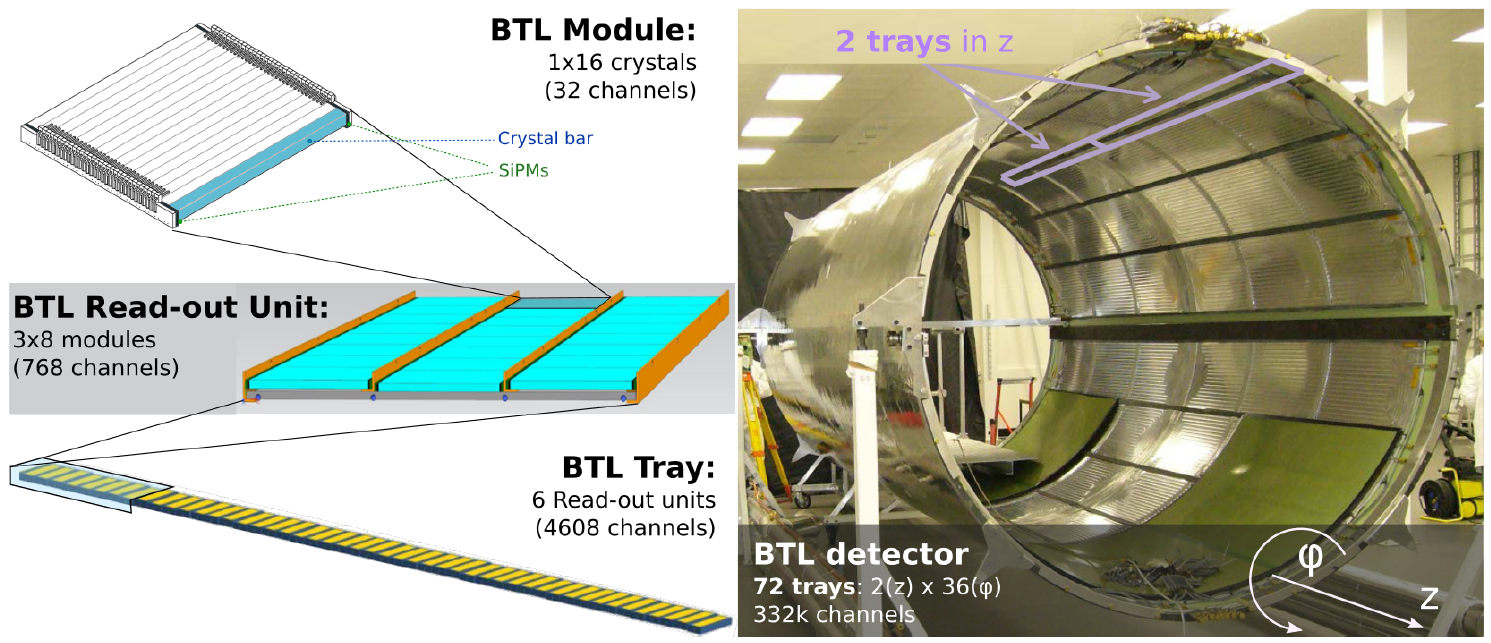
\includegraphics[width=1.0\linewidth]{Figures/BTL_overview}
 	\caption[Overview of the BTL]{On the left is an overview showing how the various components of the BTL fit together into modules, read-out units, and trays.  On the right is a view of how the trays will fit into the Tracker Support Tube (TST)}
 	\label{fig:btloverview}
 \end{figure}
 

\begin{figure}[h]
	\centering
	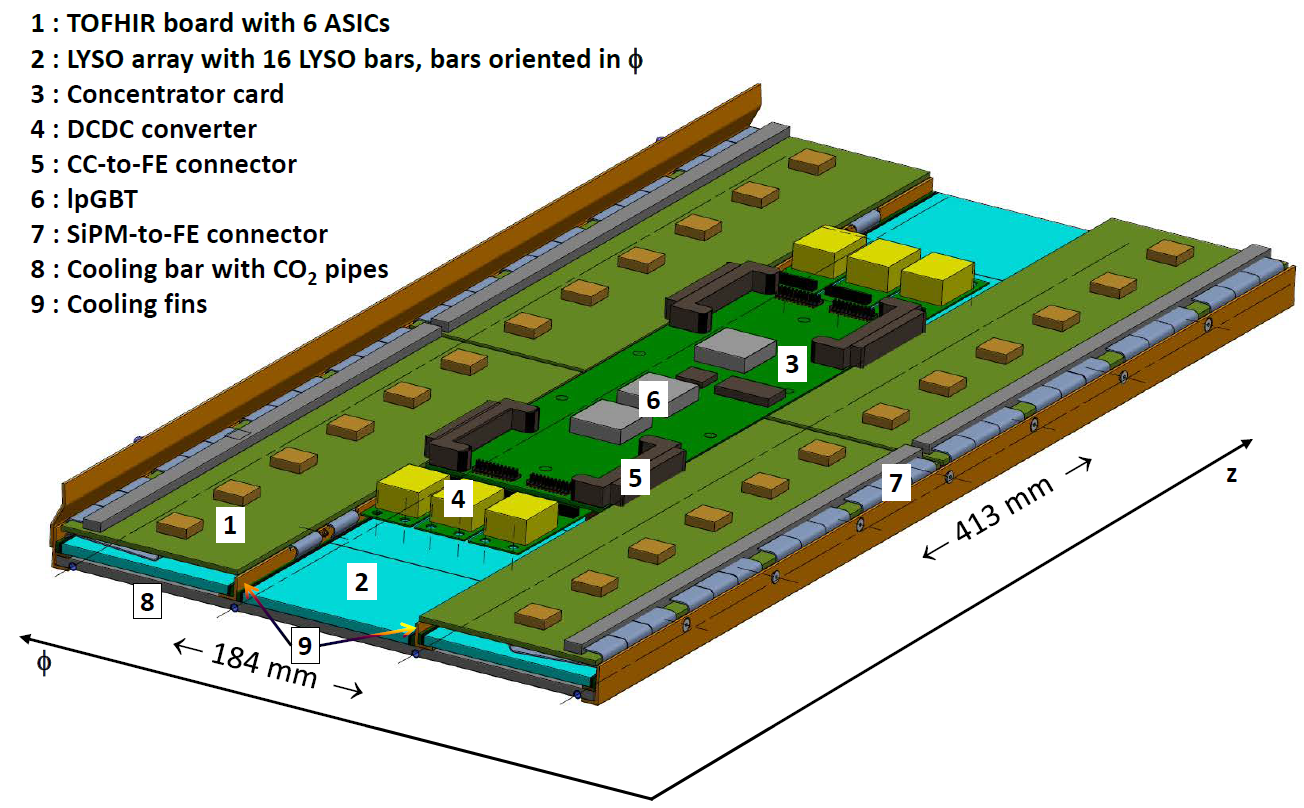
\includegraphics[width=1.0\linewidth]{Figures/BTL_readoutunit}
	\caption[Readout unit for the BTL.]{Readout unit for the BTL.}
	\label{fig:btlreadoutunit}
\end{figure}

The "time stamp" provided by the BTL is a measurement of the time that a MIP crosses the detector.  As a MIP passes through the volume of a LYSO:Ce crystal it will produce optical photons along its path.  The number of photons produced is proportional to the light yield (LY) of the crystal, which is a function of the amount of energy deposited.  Of these photons, a fraction of them will reflect along the length of the crystal bar and be detected by one of the two SiPMs mounted on the ends.  The SiPMs convert these detected photons into photoelectrons to produce electrical signals which are then processed by the TOFHIR chip to provide the "time stamp" for the MIP.  Throughout this process there are multiple contributors to time resolution degradation.  The sum of these contributions in quadrature as shown in Equation \ref{eqn:timeresolution} gives the overall time resolution for the BTL.
\begin{equation}
	\sigma_t^{BTL} = \sigma_t^{clock} \oplus \sigma_t^{digi} \oplus \sigma_t^{ele} \oplus \sigma_t^{pho} \oplus \sigma_t^{DCR}
	\label{eqn:timeresolution}
\end{equation}
The individual contributions are shown in Table \ref{table:timeres}.
\begin{table}[h]
	\centering
	\begin{tabular}{|l|c|c|}
		\hline
		Source & starting $\sigma_t$ (ps) & end-of-life (3000 fb$^{-1}$) $\sigma_t$ (ps)\\
		\hline
		Clock jitter & 15 & 15 \\
		\hline
		Digitization & 7 & 7 \\
		\hline
		Electronics & 8 & 8 \\
		\hline
		Photo-statistics & 25 & 30 \\
		\hline
		SiPM dark counts & negligible & 50 \\
		\hline
	\end{tabular}		
\label{table:timeres}
\end{table}
As one can see from this table, the two major factors in overall time resolution are photo-statistics and, at the end of life, dark counts or noise from the SiPMs.  The evolution of timing performance of the BTL as a function of the integrated luminosity is shown in Figure \ref{fig:btltimeresevolution}.  It's clear that the two most important details required to obtain and preserve good time resolution are optimizing the photo-statistics and mitigating the increased noise produced by heavily irradiated SiPMs as the integrated luminosity approaches the 3000 fb$^{-1}$ end of life target.    
\begin{figure}[h]
	\centering
	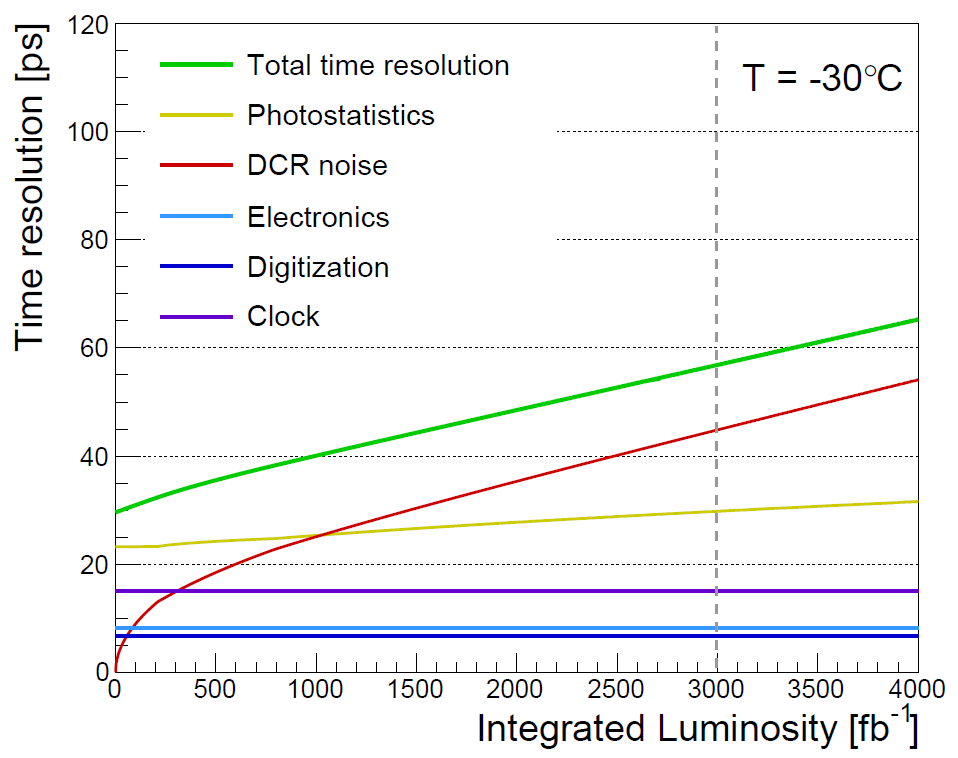
\includegraphics[width=1.0\linewidth]{Figures/btltimeres_evolution}
	\caption[Evolution of time resolution for the BTL.]{Evolution of time resolution for the BTL.}
	\label{fig:btltimeresevolution}
\end{figure}


\subsection{LYSO:Ce crystals}
As previously stated, photo-statistics has a major impact on the achievable time resolution of the BTL.  The contribution to the overall time resolution can be expressed as 
\begin{equation}
	\sigma_t^{pho} \propto \sqrt{\frac{\tau_r\tau_d}{N_{phe}}} \propto \sqrt{\frac{\tau_r\tau_d}{E_{dep}\times LY \times LCE \times PDE}},
	\label{equation:photostats}
\end{equation}
where the rise and decay times of the scintillation pulses are $\tau_r$ and $\tau_d$ respectively, $N_{phe}$ is the number of photoelectrons produced, $E_{dep}$ is the energy deposited in the crystal, $LY$ is the light yield, $LCE$ is the light collection efficiency which is the fraction of optical photons that make it down the length of the crystal to the SiPMs, and $PDE$ is the photon detection efficiency which is the fraction of photons incident on the SiPM surface that are detected.  From Equation \ref{equation:photostats} we see that an ideal candidate material for the crystals is one with fast decay and rise times, large $E_{dep}$, and high LY. LYSO:Ce has a decay time $\sim$ 40 ns and a rise time $<100$ ps \cite{Gundacker:2018tlh}.  The energy deposited by a MIP in a crystal follows a Landau distribution with the most probably value being at 0.86 MeV/mm.  For the BTL crystals a MIP deposits an average energy of 4.2 MeV when accounting for the longer path lengths within the LYSO:Ce volume due to track bending in the magnetic field.  While the LY is about 40000 photons/MeV, the most important photons are the "early photons" which are those produced in the first 500 ps of scintillation.  LYSO:Ce produces approximately 400 early photons/MeV resulting in about 2000 early photons being produced per MIP in the BTL. 

Additionally, these crystals must be tolerant to radiation levels up to those listed in Table \ref{table:fluences} with the 1.5 safety margin.  Comparing the change in transparency of LYSO:Ce after exposure to 24 GeV proton to a $2.5 \times 10^{13}$ cm$^{-2}$ fluence, which is more than the expected level including the safety margin, show a negligible loss in transparency $T$ (Figure \ref{fig:lysoradiationhard}).  At the LYSO:Ce peak scintillation wavelength of 420 nm the induced absorption coefficient is 
\begin{equation}
	\mu_{ind} = \frac{\ln(T_{before}/T_{after})}{L} = 0.5 m^{-1}
\end{equation}
where $L$ is the length of the crystal bar.
\begin{figure}[h]
	\centering
	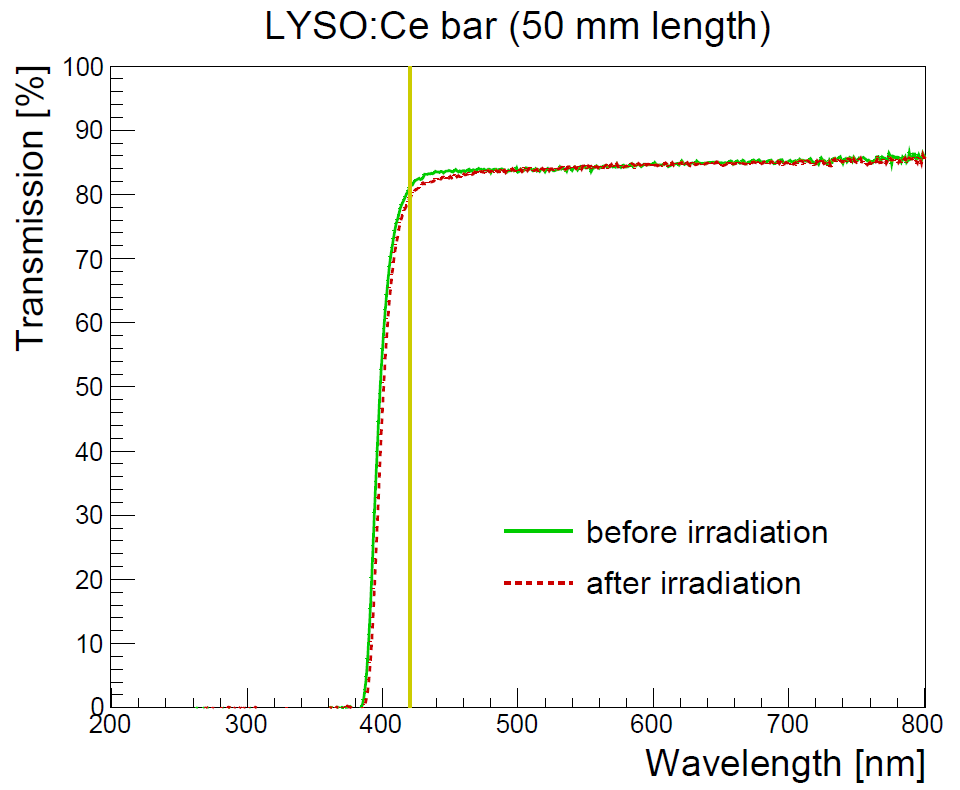
\includegraphics[width=1.0\linewidth]{Figures/LYSO_radiationhard}
	\caption[Transmission curve for LYSO:Ce before and after being irradiated to a fluence of $2 \times 10^{13}$ cm$^{-2}$ with 24 GeV protons.]{Transmission curve across a 50 mm long bar of LYSO:Ce before and after being irradiated to a fluence of $2 \times 10^{13}$ cm$^{-2}$ with 24 GeV protons.  The vertical line indicates the peak wavelength in the scintillation emission spectrum of LYSO:Ce.}
	\label{fig:lysoradiationhard}
\end{figure}
In addition to investigating the changes in optical transmission, the effect on the timing resolution was also checked to insure that the observed changes in the transmission did not have a substantial effect on the timing performance.  The time resolution before and after irradiation was measured using 511-keV photons from a Na$^{22}$ source with the results shown in \ref{fig:lysoradhardtimeres}.  This shows that there is no statistically significant change in the time resolution due to the radiation induced changes in optical transmission.  


\begin{figure}[h]
	\centering
	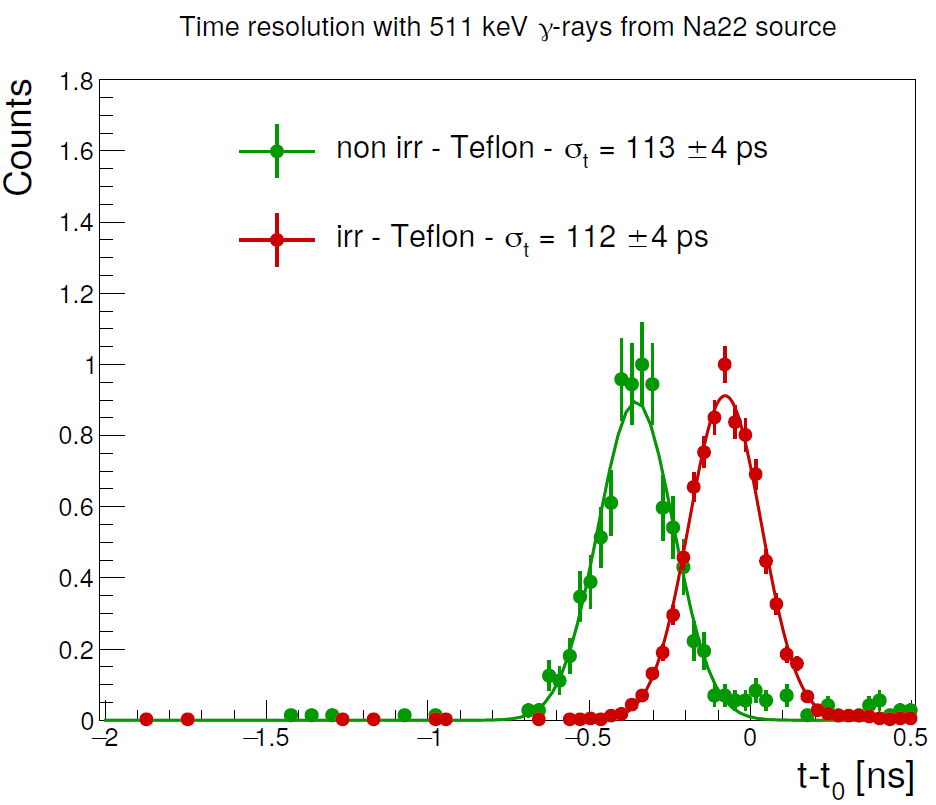
\includegraphics[width=1.0\linewidth]{Figures/lysoradhardtimeres}
	\caption[Time resolution measurements of LYSO:Ce before and after irradiation.]{The time resolution of a 50 mm long LYSO:Ce bar was measured before and after being irradiated with 24 GeV protons to a $2 \times 10^{13}$ cm$^{-2}$ fluence. The time resolution was measured using 511 keV photons from a Na$^{22}$ source. There was no significant change in time resolution after being irradiated.}
	\label{fig:lysoradhardtimeres}
\end{figure}

\subsection{SiPMs}
Silicon photomultiplier (SiPMs) were chosen as the photo-sensor to be used in the BTL.  In contrast to conventional photomultiplier tubes, SiPMs are compact, robust, and insensitive to external magnetic fields.  Several different SiPMs technologies were considered for the BTL.  Some important characteristics to consider are radiation tolerance, photon detection efficiency, power consumption, and timing performance.  In consideration were the NUV-HD (thin-epi) SiPM from Fondazione Bruno Kessler (FBK) and the S12572 and HDR2 SiPMs which are both produced by Hamamatsu Photonics (HPK).  SiPMs with a 15 $\mu$m cell size were chosen as it gave the best balance between radiation tolerance and PDE.

\subsection{Glue qualification}
The LYSO:Ce bars and SiPMs will be coupled together using an optical glue.  Preliminary glue candidates were chosen to have an index of refraction similar to that of LYSO:Ce and good optical transmission at the peak wavelength of the LYSO:Ce emission spectrum (420 nm).  These candidates were NOA-61, RTV-3145, Epotek, Polytec, BC-600, and Meltmount.  Additional constraints were that the glues be mechanically strong, capable of withstanding temperatures ranging from -40 to +60$^\circ$C, and resistant to an ionizing dose of radiation up to $\sim$50 kGy (less than 3\% loss in transparency).  As Meltmount has a melting temperature below 50$^\circ$C, it was eliminated from consideration.  The remaining glue candidates were tested for radiation hardness using a Cs$^{137}$ irradiator at the University of Virginia Medical Research Facility which provided an ionizing dose at a rate of 2 Gy/min.  The primary decay mode for Cs$^{137}$ is a beta decay to an excited state of Ba$^{137}$ which then produces a 662 keV photon when dropping into its ground state.  The energy spectrum of for Cs$^{137}$ is shown in Figure \ref{fig:caesium-137gammarayspectrum-en}.
\begin{figure}[h]
	\centering
	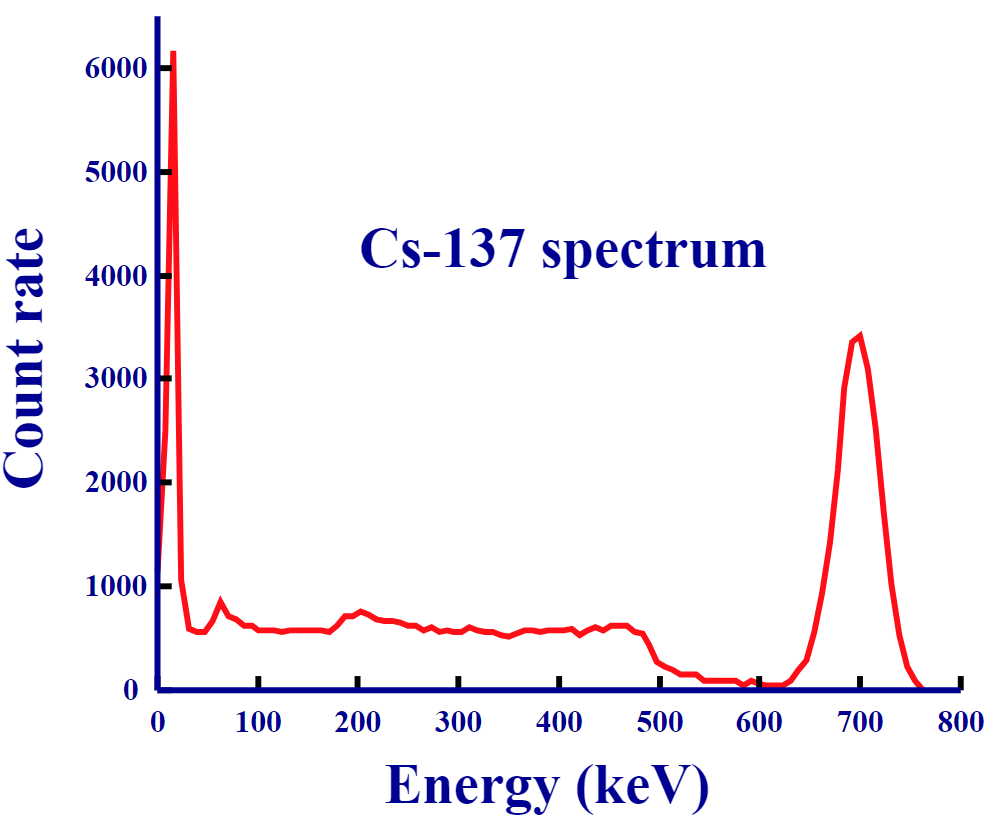
\includegraphics[width=0.7\linewidth]{Figures/Caesium-137_Gamma_Ray_Spectrum-en}
	\caption[Energy spectrum for Cs$^{137}$.]{Energy spectrum for Cs$^{137}$.}
	\label{fig:caesium-137gammarayspectrum-en}
\end{figure}
A preliminary test of radiation tolerance was performed using samples prepared by injecting glue into a teflon mold such as the one shown in Figure \ref{fig:teflonmold}.  Once cured, the glue samples (Figure \ref{fig:glueslugs})were removed from the mold and placed in the Cs$^{137}$ irradiator.  The received ionizing dose was calculated by multiplying the total time of exposure by the rate of 2 Gy/min.  The results, shown in Figure \ref{fig:gluestudies}, narrowed the list of candidates down to NOA-61 and RTV-3145.

\begin{figure}[h]
	\centering
	\subfloat[Teflon mold used to produce glue samples][Teflon mold used to produce glue samples]{
		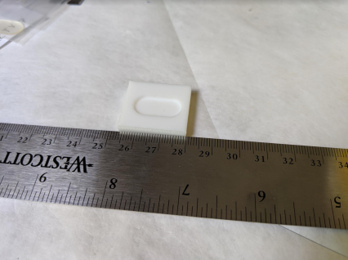
\includegraphics[width=0.4\textwidth]{Figures/teflonmold}
		\label{fig:teflonmold}}
	\qquad
	\subfloat[Glue samples][Glue samples used for preliminary radiation tolerance studies]{
		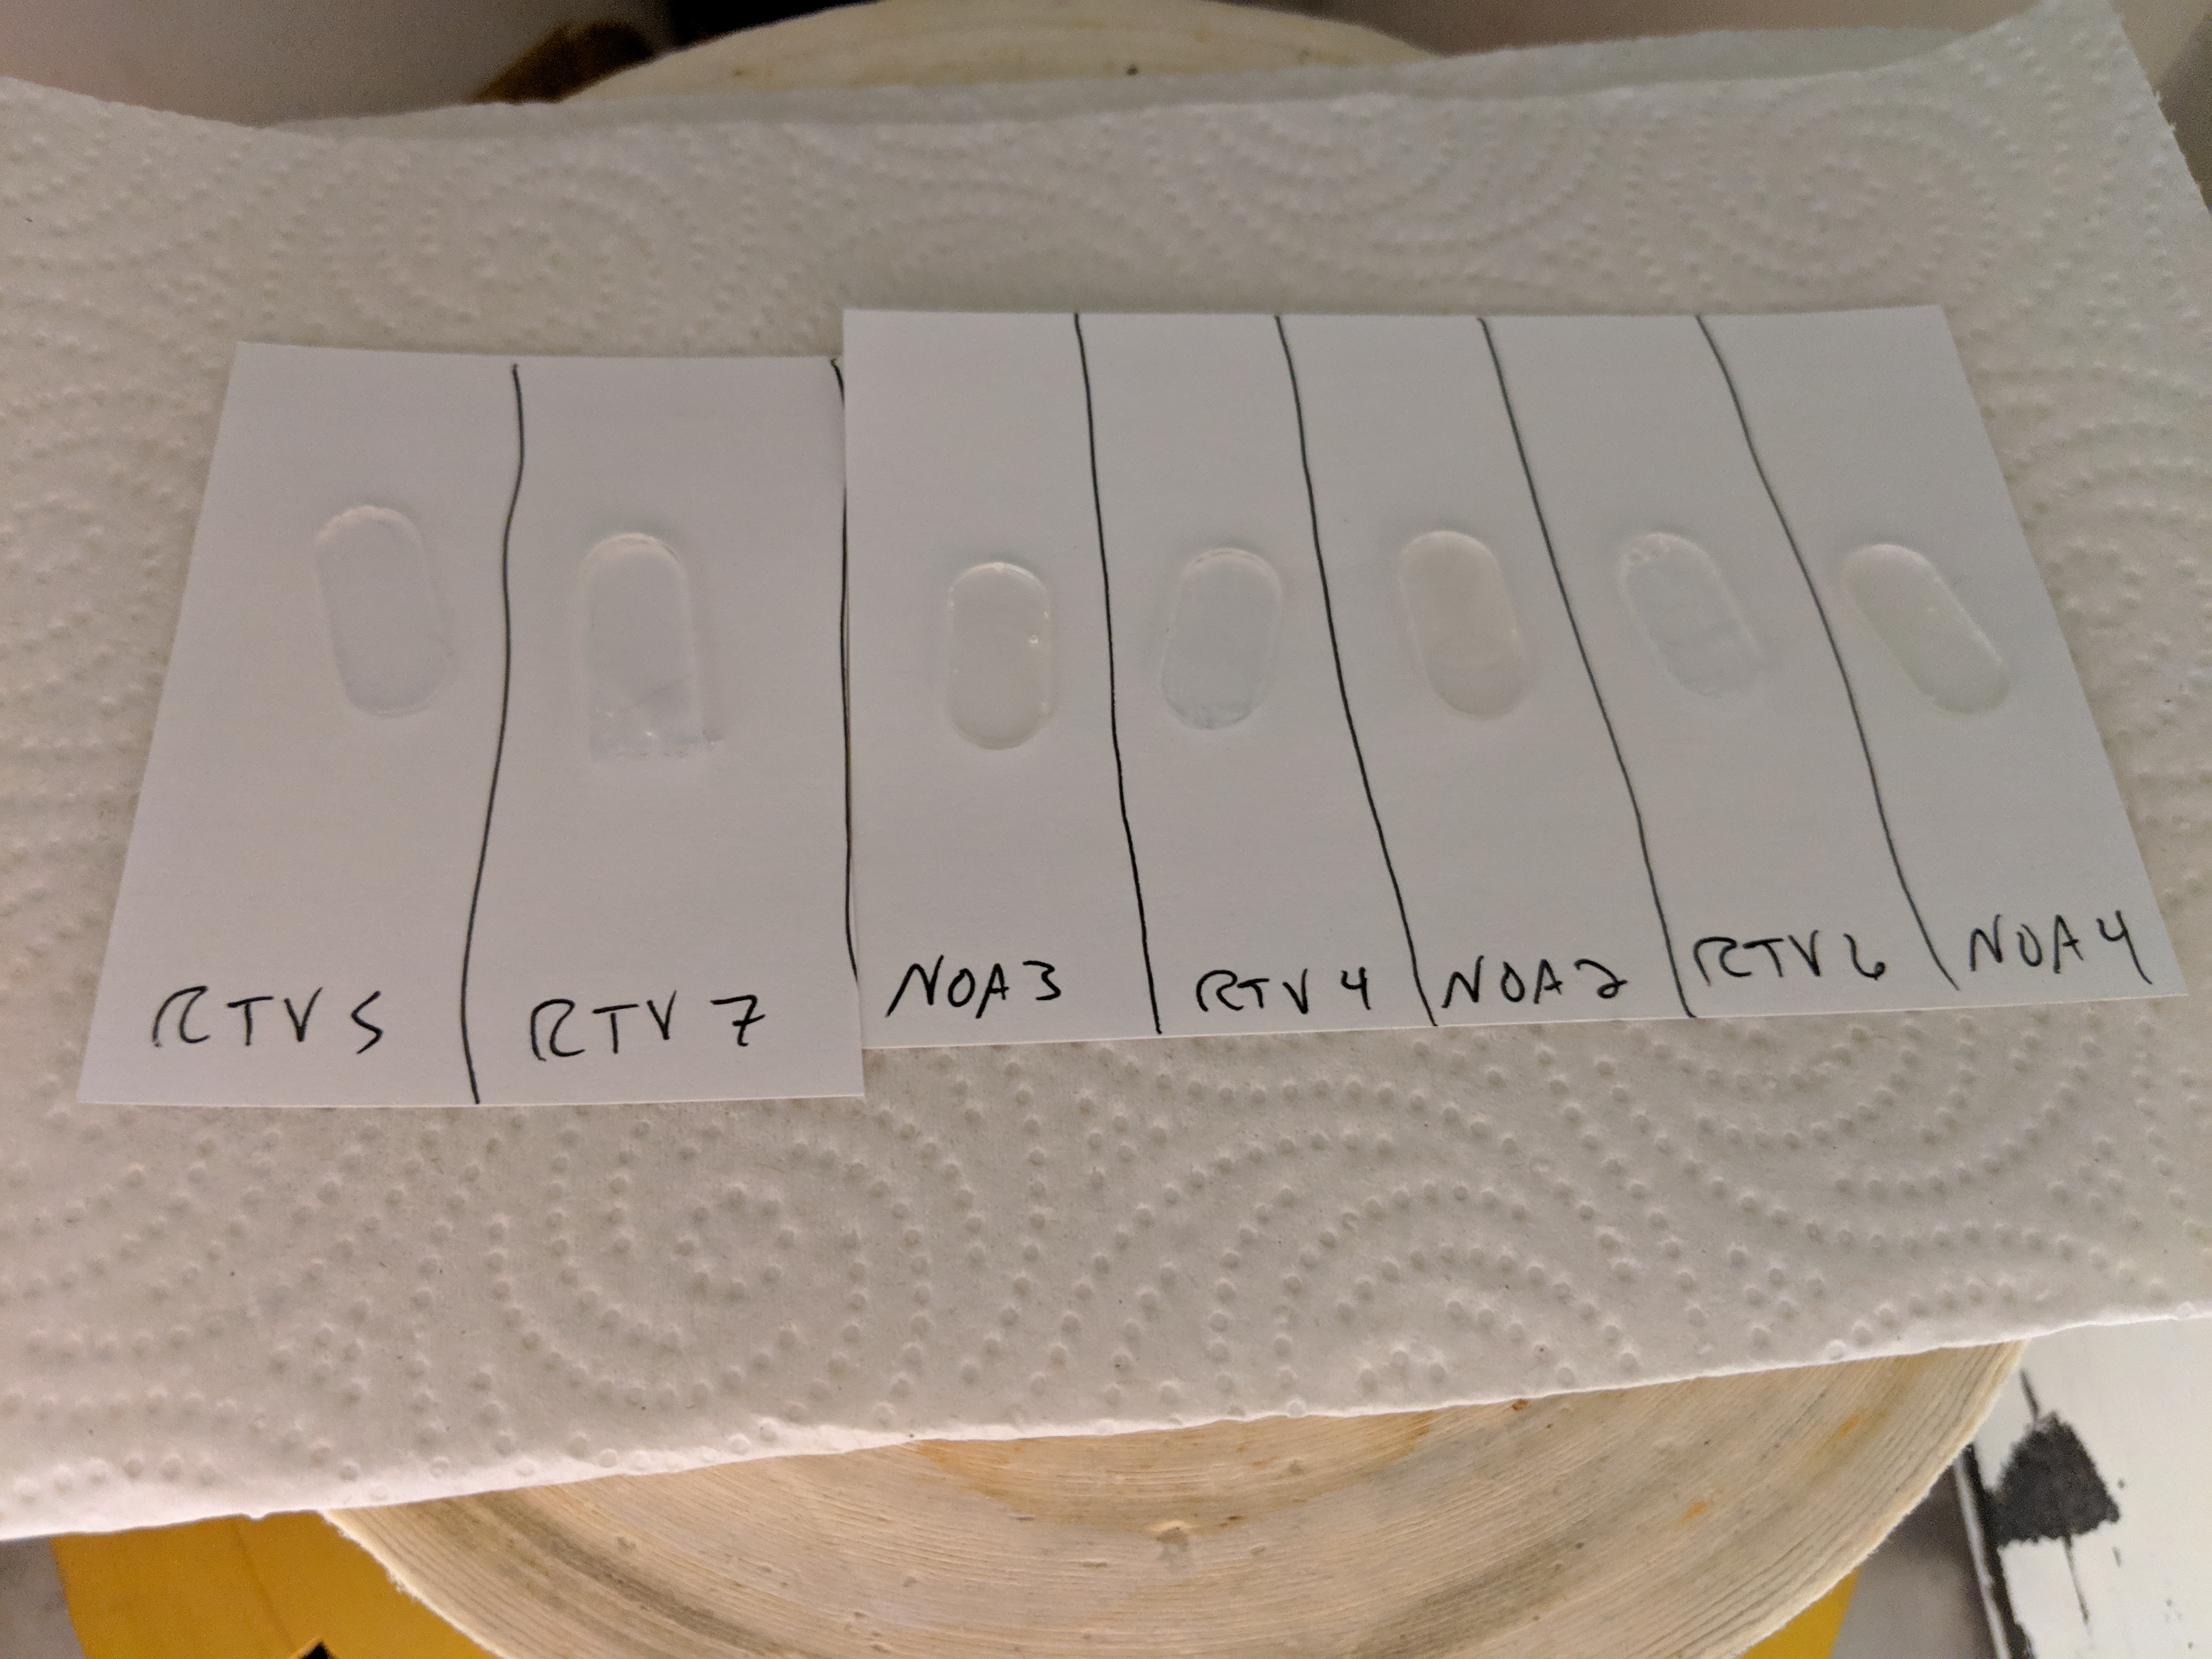
\includegraphics[width=0.4\textwidth]{Figures/glueslugs}
		\label{fig:glueslugs}}
	\label{fig:gluesampleproduction}
	\caption{Left: This is a teflon mold used to produce glue samples.  Right:  The glue samples after being removed from the mold.  These samples were then placed in the irradiator for radiation exposure.}
\end{figure}

\begin{figure}[h]
	\centering
	\subfloat[Irradiated NOA-61 glue sample][NOA-61 irradiated to 13.7 kGy]{
		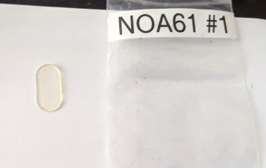
\includegraphics[width=0.4\textwidth]{Figures/noa61}
		\label{fig:noa61glue}}
	\qquad
	\subfloat[Irradiated RTV glue sample][RTV-3145 irradiated to 7.9 kGy]{
		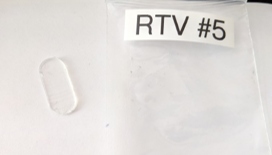
\includegraphics[width=0.4\textwidth]{Figures/rtvglue}
		\label{fig:rtvglue}}
	\qquad
	\subfloat[Irradiated Epotek glue sample][Epotek irradiated to 7.9 kGy]{
		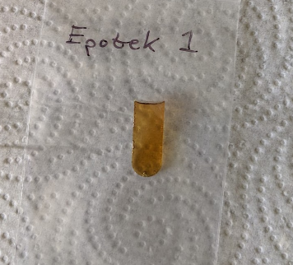
\includegraphics[width=0.4\textwidth]{Figures/epotek}
		\label{fig:epotek}}
	\qquad
	\subfloat[Irradiated Polytec glue sample][Polytec irradiated to 7.9 kGy]{
		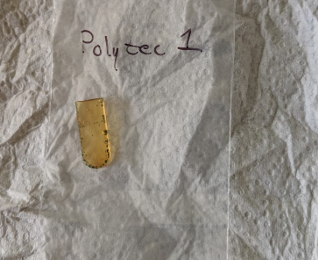
\includegraphics[width=0.4\textwidth]{Figures/polytec}
		\label{fig:polytec}}
	\quad
	\subfloat[Irradiated BC-600 glue sample][BC-600 irradiated to 10.8 kGy]{
		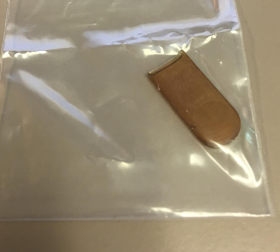
\includegraphics[width=0.4\textwidth]{Figures/bc600}
		\label{fig:bc600}}
	\caption{Preliminary radiation tolerance studies of the top five glue candidates show that only NOA-61 and RTV-3145 are viable.  Epotek, Polytec, and BC-600 all show substantial optical degradation after just a fraction of 50 kGy target.}
	\label{fig:gluestudies}
\end{figure}

At this point a more precise examination of the radiation tolerances for NOA-61 and RTV-3145 were carried out by monitoring transmission properties before and after several subsequent exposures until reaching the integrated ionizing dose of about 50 kGy.  Transmission measurements were taking using a photo-spectrometer which directs a beam of light with known wavelength through a sample and into a photo-sensor.  In order to minimize optical effects not related to radiation damage the samples need to have uniform thickness and surfaces that are both smooth and parallel.  To accomplish this the glue samples for this test were prepared by placing glue between two 1-mm thick quartz tiles which were separated by 1-mm thick spacers.  The quartz provided smooth surfaces while the spacers insured uniform glue thicknesses and parallel surfaces.  
\begin{figure}[h]
	\centering
	\subfloat[Glue sample between quartz slides][Glue sample between two quartz slides]{
		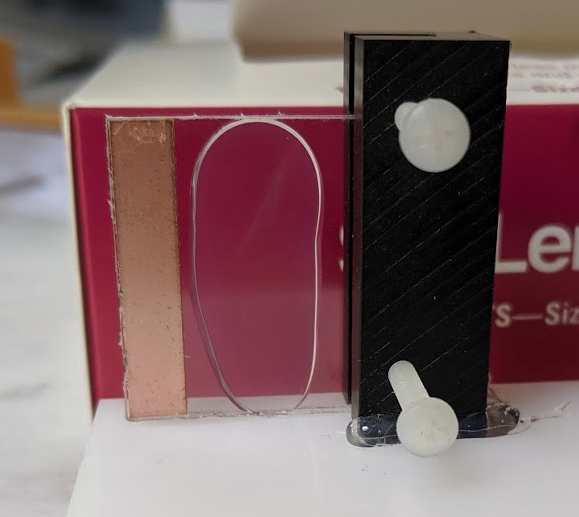
\includegraphics[width=0.4\textwidth]{Figures/quartzslidewithholder}
		\label{fig:quartzslidewithholder}}
	\qquad
	\subfloat[Glue sample positioned in photo-spectrometer][Glue sample positioned in photo-spectrometer]{
		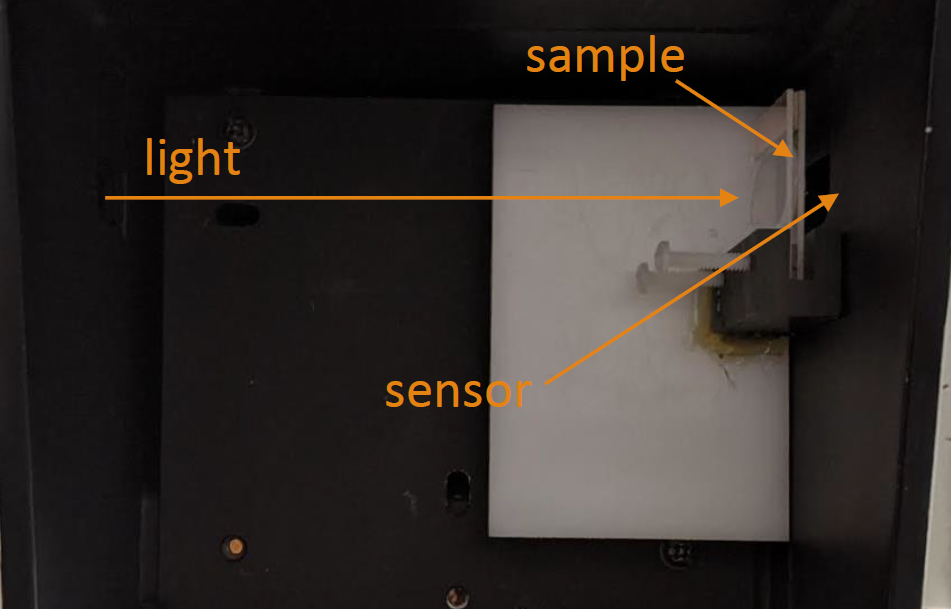
\includegraphics[width=0.4\textwidth]{Figures/photospec}
		\label{fig:photospec}}
	\caption{Figure \ref{fig:quartzslidewithholder} shows an example a glue sample ready for transmission measurements.  Figure \ref{fig:photospec} shows how the measurement is taken with the sample placed inside the photo-spectrometer.}
	\label{fig:transmissionsetup}
\end{figure}
Separate transmission measurements were taken with bare quarts tiles that were irradiated alongside the glue samples and showed negligible optical degradation.  The transmission curves for both NOA-61 and RTV-3145 are shown in Figure \ref{fig:transmissioncurves}.  The comparison of their performance at a wavelength of 420 nm (the peak of the LYSO:Ce emission spectrum) is shown in \ref{fig:transmissionat420}.  NOA-61 provides better performance prior to irradiation but degrades as the ionizing dose increases.  RTV-3145 is less affected and despite starting with a lower transmission ends up with a higher transmission after the full ionizing dose.  With the expected thickness of the glue layers in the BTL to be 50 $\mu$m or thinner, both glues would have less than 3\% loss in transparency and therefore meet the radiation tolerance requirement.

\begin{figure}[h]
	\centering
	\subfloat[Optical transmission curves for NOA-61 with increasing doses of radiation.][Optical transmission curves for NOA-61 with increasing doses of radiation]{
		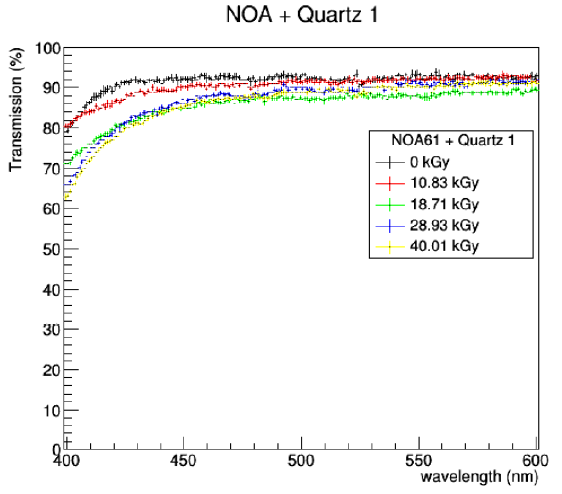
\includegraphics[width=0.5\textwidth]{Figures/noatransmission}
		\label{fig:noatrasmission}}
	\qquad
	\subfloat[Optical transmission curves for RTV-3145 with increasing doses of radiation.][Optical transmission curves for RTV-3145 with increasing doses of radiation]{
		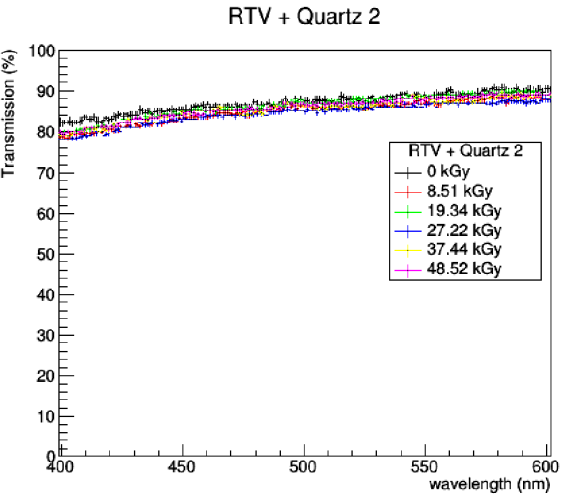
\includegraphics[width=0.5\textwidth]{Figures/rtvtransmission}
		\label{fig:rtvtransmission}}
	\quad
	\subfloat[Transmission at at wavelength of 420 nm after various ionizing doses][Transmission at at wavelength of 420 nm after various ionizing doses]{
		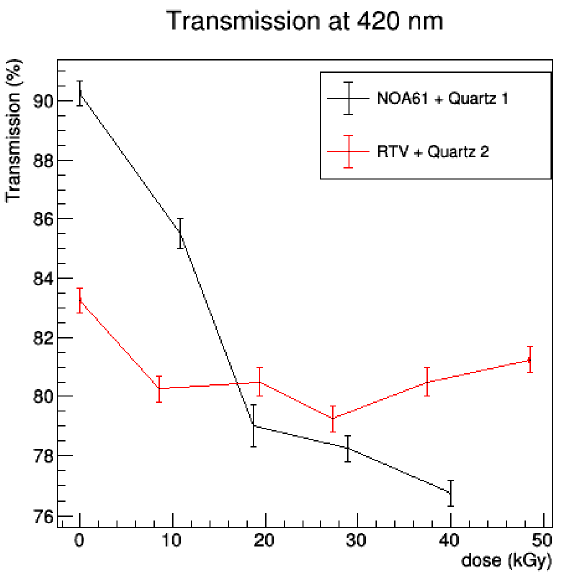
\includegraphics[width=0.5\textwidth]{Figures/transmissionat420}
		\label{fig:transmissionat420}}
	\caption{Transmission curves for both NOA-61 (Figure \ref{fig:noatrasmission} and RTV-3145 (Figure \ref{fig:rtvtransmission}).  Figure \ref{fig:transmissionat420} shows the transmission at 420 nm, the peak of the LYSO:Ce emission spectrum, with increasing ionizing doses.  While NOA-61 starts with a higher transmission, RTV-3145 is more radiation tolerant and has a higher transmission after the full ionizing dose.}
	\label{fig:transmissioncurves}
\end{figure}

As previously mentioned, the glues would need to withstand temperature ranges from -40 to +60$^\circ$C.  This was checked by gluing pairs of SiPMs to a crystal bar and thermally cycled several times between the aforementioned temperatures.  Neither glue showed visible transparency loss nor did they show any signs of structural degradation such as cracks.  The bond created by both glues remained mechanically strong.  The SiPMs glued with NOA-61 could not be removed from the crystal bar without severely damaging the SiPMs.  Those glued with RTV-3145 could be removed but only by applying a large amount of torsion.  As it is, both glues remain potential candidates as they have both surpassed the standards required for usage in the BTL.  RTV-3145 is slightly favored as it was used in the CMS ECAL with good results and has been shown to be more radiation tolerant than NOA-61.  Another benefit of RTV-3145 over NOA-61 is that the crystal bars will be covered in a wrapping prior to gluing.  This is problematic for NOA-61 because it requires exposure to UV light in order to cure and this is made difficult by the opaque wrapping.  

\subsection{Performance at test beam}

Test beam facilities at both CERN and Fermilab were used to test the BTL sensor prototypes throughout the research and development process.  These facilities provide well calibrated sources of MIPs in the form of high energy pions at CERN and protons at Fermilab.  

%Among the first test beam campaigns was an investigation of potential LYSO:Ce geometries and SiPM arrangements.  Figure \ref{fig:testbeam1} shows three configurations.  All of these configuration used HBK S12572 SiPMs having a $3 \times 3$ mm$^2$ sensitive area and 15 $\mu$m cell pitch.  These were, from left to right, a $5 \times 3 \times 3$ mm$^3$ bar with one SiPM on each end, a $5 \times 5 \times 3$ mm$^3$ tile with an array of three SiPMs on each side, and a $5 \times 5 \times 3$ mm$^3$ tile with a single SiPM centered on the back.  The crystals were wrapped in Teflon to limit external light leakage.  The time resolution for the tiles showed impact point position dependence while using the average time between the two SiPMs on the bar showed 

%\begin{figure}[h]
%	\centering
%	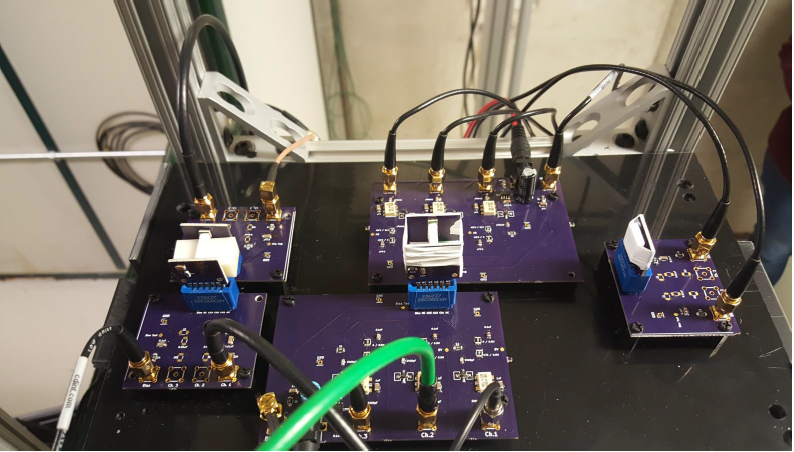
\includegraphics[width=0.7\linewidth]{Figures/testbeam1}
%	\caption[Test beam setup at Fermilab for investigating different BTL sensor configurations.]{Three BTL sensor configurations investigated during a test beam campaign at Fermilab. On the left is a $5 \times 3\times 3$ mm$^3$ LYSO:Ce bar instrumented with SiPMs on both ends. In the middle is a $5 \times 5 \times 3$ mm$^3$ tile with an array of three SiPMs on each side. To the right is $5 \times 5 \times 3$ mm$^3$ tile with a single SiPM in the middle behind the tile.}
%	\label{fig:testbeam1}
%\end{figure}


%\begin{figure}[h]
%	\centering
%	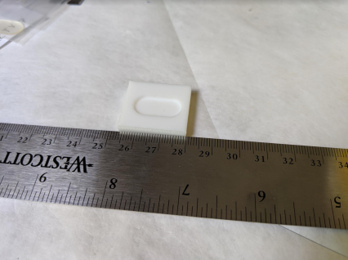
\includegraphics[width=0.7\linewidth]{Figures/teflonmold}
%	\caption[Teflon mold used for making glue samples for irradiation tests.]{Teflon mold used for making glue samples for irradiation tests.}
%	\label{fig:teflonmold}
%\end{figure}








%As mentioned above, the fundamental active element in the BTL is a thin scintillating bar made of Lutetium Yttrium Orthosilicate crystals doped with Cerium ($(Lu_{1-X}Y_X)_2SiO_5:Ce$) which is referred to as LYSO:Ce.  The bars are 57 mm long, 3.12 mm wide, and have an average thickness of 3 mm.  A silicon photomultiplier (SiPM) is attached to each end of the LYSO:Ce bar.  This double-ended readout gives uniform time response along the length of the crystal and the ability to extract positional information for tracking.  


